\chapter{Results} \label{chap:results}

In this chapter, we talk about the results. We start of by talking about the results achieved with different parameters during implementation and which we decided to use in the end. We then proceed to evaluate

If we were to assume a single-color image map obtained by spectrally rendering one atlas entry and we were to uplift a pixel of this image map, it would be crucial for its position in the RGB cube to be the closest to a lattice point seeded by the original atlas entry, so as to utilize it during uplifting. Even a slight change in the RGB value of the image map may cause the uplifting to consider different point as primary during interpolation, which could lead to undesired behavior. Additionaly, especially in the cases of a low voxel size (i.e. high cube \texttt{dimension} parameter), such a change could even cause the pixel of the image map to be uplifted in a different voxel than the original atlas entry, which might possibly not utilize the atlas entry at all. As the variance in the RGB value of the resulting image map is inevitable due to the stochastic nature of the spectral rendering process, - navyse daco s tymto spravit

\section{Implementation parameters}

\subsection{Storing moments} \label{sec:storingMoments}

The first thing we analyze and decide on is the technique used for mapping wavelengths to a signal for the storage and subsequent reconstruction of moments. As already mentioned in~\cref{par:spectrumToCoefficientConversion}, we have the choice of both \emph{mirroring} and \emph{warping} the signal, which overall creates four options --- using only mirroring, using only warping, using both or using neither, i.e. utilizing the original signal.

Note that, although we aim for the highest possible precision in terms of curve reconstruction for the atlas lattice points, so as to lose as little information about the original atlas entry as possible, this is not the case for regular lattice points. On the contrary --- as they do not have a prior atlas entry that their spectra must approximate, we mainly aim for their smoothness in order to prevent color artifacts upon interpolation.

Additionally, when choosing the correct wavelength mapping technique, we must also take the performance of the optimizer under it into account.

We start by focusing on the accuracy of reconstruction for the atlas lattice points. We run an experiment across multiple color atlases (such as the Pantone atlas, Munsell Book of Colors or RAL atlas) and multiple illuminants in which we compare the original color of spectral curve under an illuminant with the color of a spectrum obtained by reconstruction from the original curve's coefficients under said illuminant. We then compute the average and maximum obtained color difference. For these purposes, we use the simple Delta E error due to its continuous nature.

In~\cref{sec:completeMomentError}, we provide all results obtained from these experiments. Note that using $n$ moments requires storing $n+1$ values in case mirroring is used (i.e. the moments are real) and $2n+1$ values otherwise (i.e. the moments are complex). As we are interested in the number of $coefficients$ needed for storage (and for passing to the optimizer) rather than the number of moments, we surmise the contents of~\cref{sec:completeMomentError} in~\cref{table:comparisonMomentTechnique}, where we present the errors according to the number of coefficients.

\begin{table}[t]
	\centering
	\begin{tabular}{crrrrrrrr}
		\toprule
		\multirow{4}{*}{Coefficients} &
		\multicolumn{8}{c}{Methods} \\
		\cmidrule(lr){2-9}
		&\multicolumn{2}{c}{M\&W} &
		\multicolumn{2}{c}{M\&nW} &
		\multicolumn{2}{c}{nM\&W} &
		\multicolumn{2}{c}{nM\&nW}\\
		\cmidrule(lr){2-9}
		& Avg & Max & Avg & Max & Avg & Max & Avg & Max \\
		\cmidrule(lr){1-9}
		1&24.37&202.43&24.21&202.57&24.27&202.47&24.21&202.57\\
		2&12.77&151.47&16.77&162.39&\textemdash&\textemdash&\textemdash&\textemdash\\
		3&1.71&28.28&10.23&115.27&4.03&72.86&8.39&101.6\\
		4&0.96&13.66&6.11&93.14&\textemdash&\textemdash&\textemdash&\textemdash\\
		5&0.65&10.51&2.52&38.34&1.3&28.31&2.65&30.48\\
		6&0.47&7.13&1.44&10.4&\textemdash&\textemdash&\textemdash&\textemdash\\
		7&0.43&5.7&0.97&10.47&0.75&10.81&1.1&9.58\\
		8&0.38&5.29&0.85&9.8&\textemdash&\textemdash&\textemdash&\textemdash\\
		9&0.37&5.02&0.69&6.55&0.64&7.06&0.58&5.97\\ 
		10&0.25&4.48&0.51&6.2&\textemdash&\textemdash&\textemdash&\textemdash\\
		11&0.25&4.28&0.34&4.21&0.49&4.62&0.49&5.23\\
		12&0.19&4.09&0.27&4.15&\textemdash&\textemdash&\textemdash&\textemdash\\
		13&0.19&3.92&0.26&3.83&0.31&2.97&0.37&4.88\\
		14&0.19&3.66&0.25&3.75&\textemdash&\textemdash&\textemdash&\textemdash\\
		15&0.19&3.45&0.23&3.58&0.3&2.98&0.34&3.89\\
		16&0.16&3.18&0.2&2.94&\textemdash&\textemdash&\textemdash&\textemdash\\
		17&0.16&3.07&0.19&2.32&0.28&2.49&0.3&2.6\\
		18&0.16&2.94&0.16&1.78&\textemdash&\textemdash&\textemdash&\textemdash\\
		19&0.16&2.84&0.15&1.94&0.26&2.83&0.22&2.65\\
		20&0.16&2.72&0.15&1.76&\textemdash&\textemdash&\textemdash&\textemdash\\
		21&0.16&2.6&0.15&2.0&0.26&2.65&0.22&2.75\\
		\bottomrule
	\end{tabular}
	\caption{The average and maximum \emph{Delta E} error originating from round-trips under multiple illuminants. $M$ represents mirroring, $W$ warping, and the symbol $n$ stands for their negation.}
	\label{table:comparisonMomentTechnique}
\end{table}

By observing~\cref{table:comparisonMomentTechnique}, we conclude that it is beneficial to mirror the signal. Although the non-mirroring technique performs slightly better for $c \le 9$, we are looking for a technique with which to save even the most complicated spectra which requires a lot more coefficients, and for that, non-mirroring is insufficient.

By applying the same principle when choosing whether to warp the signal, we assume that warping should provide better results. However, as the results from~\cref{table:comparisonMomentTechnique} are not entirely clear on this matter, as for $c \ge 16$, the maximum error of non-warping is lower, we put this theory to practice and test the performance of the optimizer with both warping and non-warping. 

To achieve a certain color error upon reconstruction, the warping technique usually requires less coefficients. To give an example, if we require Delta E to be $\Delta E_{ab}^*=0.1$ under the FL11 illuminant, the Munsell Book of Colours requires 14 coefficients on average with warping and 18 if not.

Even despite the benefit of having less coefficients to optimize, the average distance between the original and the fitted curves when using either of the cost functions (presented in~\cref{ssec:costFunctions}) is higher for warping. This does necessarily need to imply failure --- as the edges of the curve do not often bear significant color information, we do not require them to be reconstructed as precisely. However, occasionally, the optimizer fails in so as the fitted curve does not follow the original at all but rather ends up as a spiky spectrum susceptible to metameric artifacts. We show some of these results in~\cref{fig:warping_atlasLatticePoints}, where we compare them to the results with the non-warping technique.

\begin{figure}[t]
	\centering
	\captionsetup[subfigure]{font=footnotesize,labelfont=footnotesize}
	\captionsetup[subfigure]{justification=centering}
	\begin{subfigure}[t]{0.38\textwidth}
		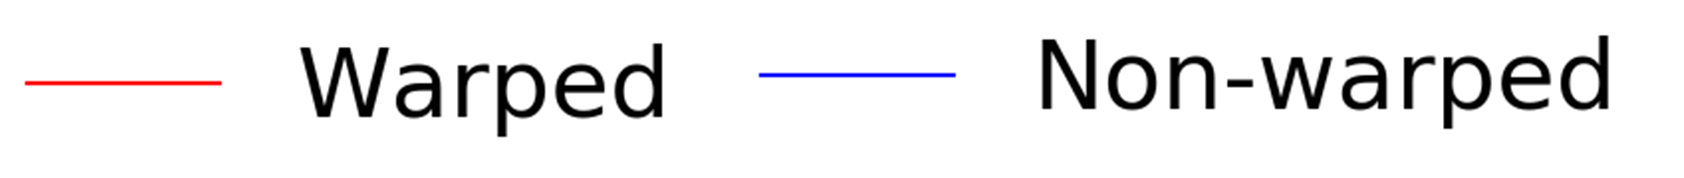
\includegraphics[width=\linewidth]{img/resultsTechniqueOpt_legend.png}
	\end{subfigure} \\
	\begin{subfigure}[t]{0.32\textwidth}
		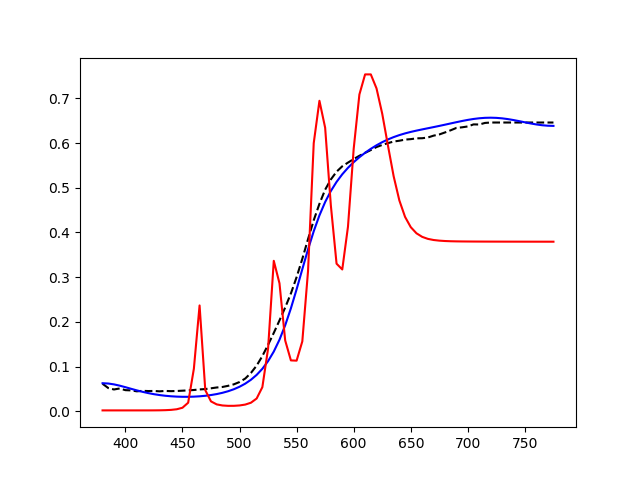
\includegraphics[width=\linewidth]{img/results_warping_orange.png}
		\caption{``orange'' patch}
		\label{fig:warping_alp_neutral50}
	\end{subfigure} \hspace{0.1em}
	\begin{subfigure}[t]{0.32\textwidth}
	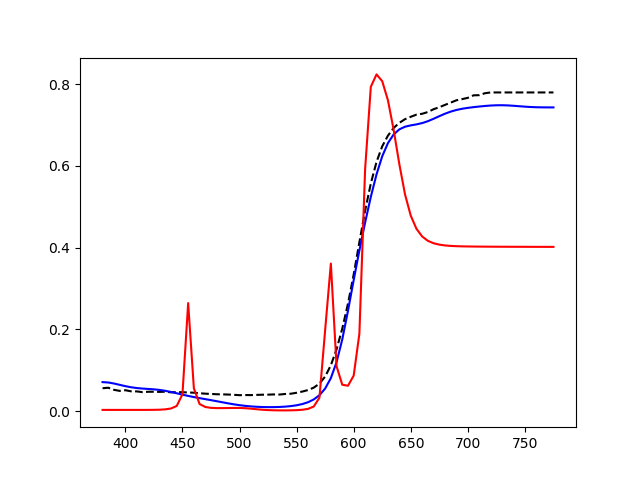
\includegraphics[width=\linewidth]{img/results_warping_red.png}
	\caption{``red'' patch}
	\label{fig:warping_alp_red}
	\end{subfigure} \hspace{0.1em}
	\begin{subfigure}[t]{0.32\textwidth}
		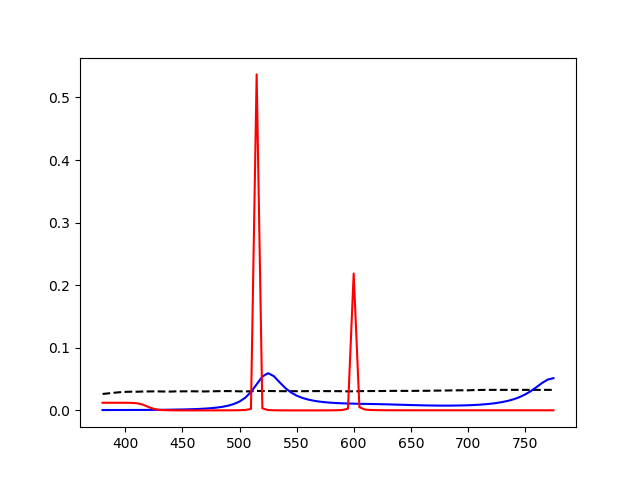
\includegraphics[width=\linewidth]{img/results_warping_black.png}
		\caption{``black'' patch}
		\label{fig:warping_alp_black}
	\end{subfigure}
	\caption{Failure of warping when fitting atlas lattice points, shown on patches from the Macbeth Color Chart}
	\label{fig:warping_atlasLatticePoints}
\end{figure}

For the regular lattice points, we present a similar comparison in~\cref{fig:warping_regularPoints}, where we seed cubes of different sizes with distinct atlases and analyze the spectra at specific points. Not warping the signal is superior to warping even in this case, as it creates smoother spectra with less sharp edges. 

As we eventually decide on using only 3 coefficients per regular lattice points (see~\cref{ssec:noOfMoments}), and for that purpose, even warping works reasonably well, we proba

Although we eventually decide on using only 3 coefficients per regular lattice points, and for that purpose, even warping performs reasonably well, we conclude that not warping the signal is by far superior.

\begin{figure}[t]
	\centering
	\captionsetup[subfigure]{font=footnotesize,labelfont=footnotesize}
	\captionsetup[subfigure]{justification=centering}
	\begin{subfigure}[t]{0.38\textwidth}
		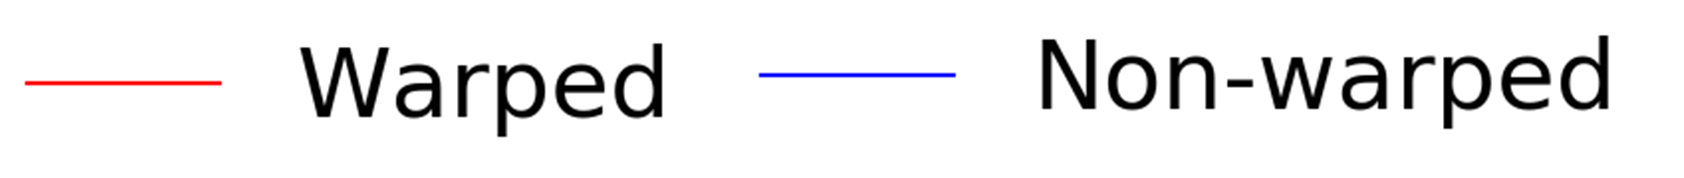
\includegraphics[width=\linewidth]{img/resultsTechniqueOpt_legend.png}
	\end{subfigure} \\
	\begin{subfigure}[t]{0.31\textwidth}
		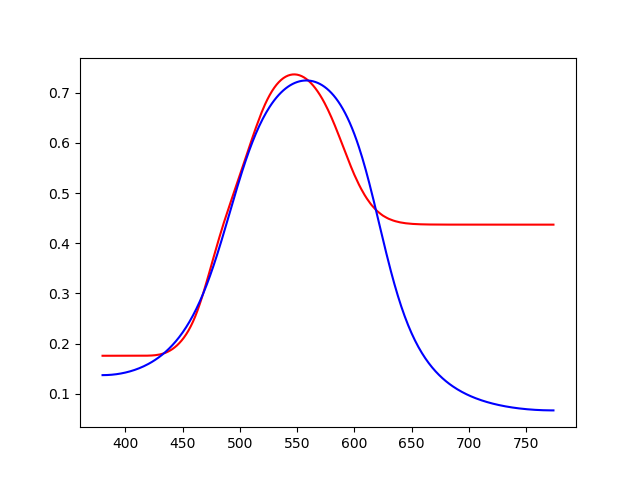
\includegraphics[width=\linewidth]{img/resultsTechniqueOpt_m3_cd64.png}
		\caption{$c=3, cd=64$,\\$RGB=(222.6, 230.7, 230.7)$,\\initial atlas = Macbeth Color Chart}
		\label{fig:warping_regularPointst_m3_cd64}
	\end{subfigure}
	\begin{subfigure}[t]{0.31\textwidth}
		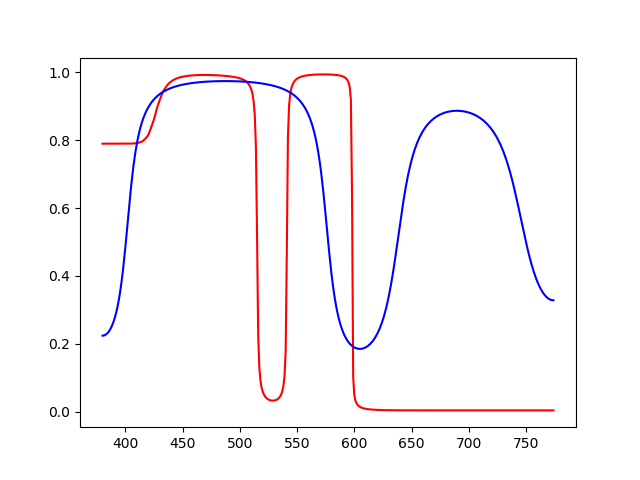
\includegraphics[width=\linewidth]{img/resultsTechniqueOpt_m5_cd32.png}
		\caption{$c=5, cd=32$,\\$RGB=(82.26, 172.74, 255)$,\\initial atlas = Page 14 from Munsell Book of Color}
		\label{fig:warping_regularPoints_m5_cd32}
	\end{subfigure}
	\begin{subfigure}[t]{0.31\textwidth}
		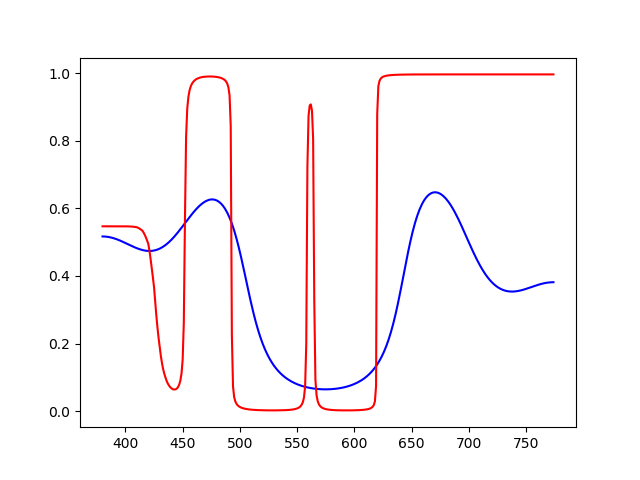
\includegraphics[width=\linewidth]{img/resultsTechniqueOpt_m7_cd16.png}
		\caption{$c=7, cd=16$,\\$RGB=(102, 17, 153)$,\\ fitted from middle}
		\label{fig:warping_regularPoints_m7_cd16}
	\end{subfigure} 
	\caption{Comparison of warping and non-warping when used for fitting regular atlas entries. Note that the figures are illustrative, as they were created with an older version of the cube and therefore may not correspond to the current results.}
	\label{fig:warping_regularPoints}
\end{figure}

We accredit the shortcomings of warping to its fixation on proper reconstruction of the middle part of the curve and its neglect of the edges. Since the 


 Since warping focuses on the more important regions of the spectrum in terms of color perception (i.e. around 550nm), it reconstructs the slight waves in this area quite precisely while neglecting the edges. Therefore, 

 Non-warping, on the other hand, focuses on the spectra as a whole, which results in approximating the shape over the whole wavelength range but not in an exact replication of any specific spikes.

We conclude that our theory is correct --- warping indeed amplifies the slight differences around the middle of the curve in order to achieve the correct color, so much that it creates spikier spectra the more the cube grows. Although this does not necessarily render the cubes created with warped signal useless, it is apparent they are prone to creating memateric artifacts such as the ones presented in~\cref{fig:metamerism}. Additionally, as we already mentioned in ref, the interpolation phase of the rendering pipeline benefits from smooth, non-spiky spectra, which is a criterion the warped spectra do not satisfy. Therefore, we it is save to discard the option of warping.






\begin{figure}[t]
	\centering
	\captionsetup[subfigure]{font=footnotesize,labelfont=footnotesize}
	\captionsetup[subfigure]{justification=centering}
	\begin{subfigure}[t]{0.60\textwidth}
		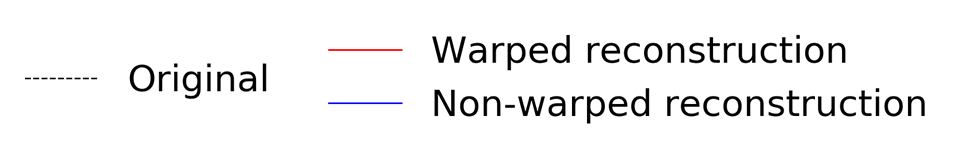
\includegraphics[width=\linewidth]{img/results_techniqueLegend.png}
	\end{subfigure} \\
	\begin{subfigure}[t]{0.45\textwidth}
		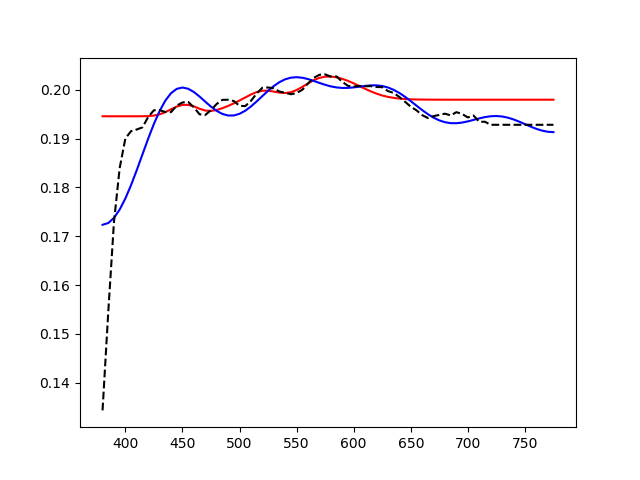
\includegraphics[width=\linewidth]{img/results_techniqueNeutral5.png}
		\caption{``neutral 5'' patch}
		\label{fig:resultsTechnique_neutral5}
	\end{subfigure} \hspace{0.1em}
	\begin{subfigure}[t]{0.45\textwidth}
		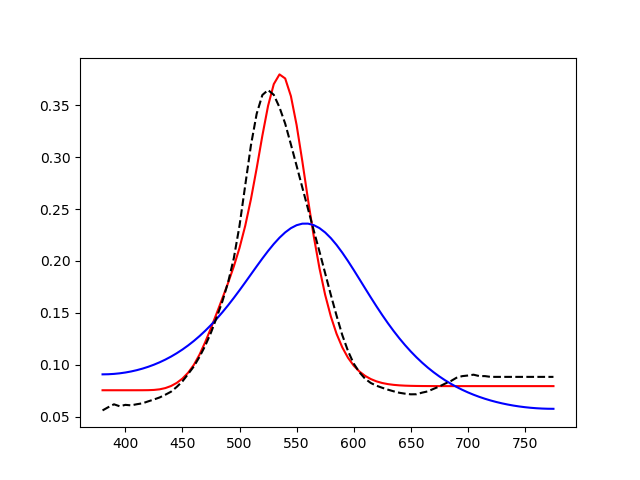
\includegraphics[width=\linewidth]{img/results_techniqueGreen.png}
		\caption{``green'' patch}
		\label{fig:resultsTechnique_green}
	\end{subfigure} \hspace{0.1em}
	\vspace{0.5em}\\
	\begin{subfigure}[t]{0.45\textwidth}
		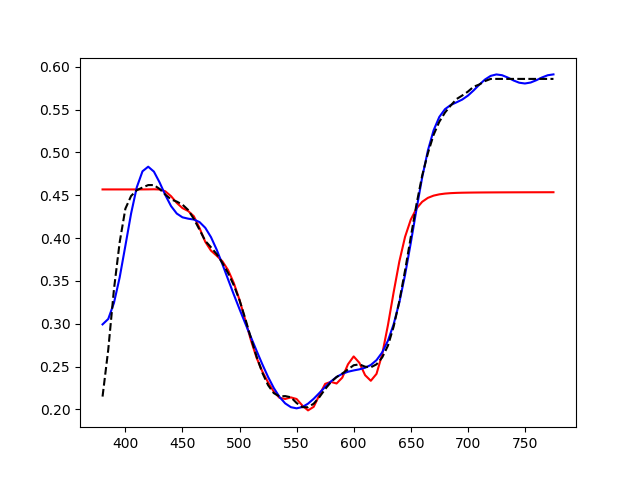
\includegraphics[width=\linewidth]{img/results_techniqueBlueFlower.png}
		\caption{``blue flower'' patch}
		\label{fig:resultsTechnique_blueFlower}
	\end{subfigure} \hspace{0.1em}
	\begin{subfigure}[t]{0.45\textwidth}
		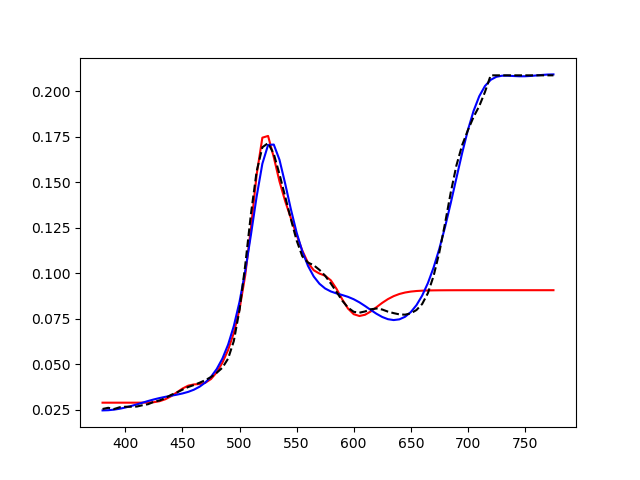
\includegraphics[width=\linewidth]{img/results_techniqueFoliage.png}
		\caption{``foliage'' patch}
		\label{fig:resultsTechnique_foliage}
	\end{subfigure}
	\caption{Comparison between the warped and non-warped reconstructed signal shown on multiple patches of the Macbeth Color Chart}
	\label{fig:resultsTechniques}
\end{figure}


Although the shortcomings of warping can already be perceived in e.g.~\cref{fig:resultsTechnique_foliage} or~\cref{fig:resultsTechnique_blueFlower}, the failure in the reconstruction of the curve's edges does not have a significant effect of the the resulting RGB color, as the source of color is mainly focused around the middle of the curve. However, if the edges are extremely distinct from the rest of the curve (see~\cref{fig:resultWorstWarp}), they tend to provide unanticipated color information. In such cases, warping the signal presents a disadvantage.

Obviously, the Delta E error caused by unnecessary warping can be reduced to almost 0 by passing the computed coefficients to the optimizer, which then alters the curve so that it evaluates to the correct RGB. However, because we lose the notion of the curve's desired shape and because warping does not focus on the edges, the optimizer is apt to amplify the already existing slight bumps in the middle. This behavior may therefore cause the resulting shape to be extremely distinct from the desired one. 

The non-warping technique, shown in~\cref{fig:resultWorstNonWarp}, is not susceptible to this kind of behavior. Although it creates a rather significant Delta E error, we can observe that the shape of the reconstructed spectrum roughly resembles the original shape. Such a behavior is desired in our case, as the reconstructed reflectance is less prone to cause metameric artifacts under different illuminants. Additionally, as the non-warping technique forces the optimizer to not prioritize specific parts of the curve, the optimization is prone to slightly altering the shape as a whole rather than creating 
irregularities in the middle. Therefore, regardless of the average error, we assume the non-warping technique to outperform warping both when performing simple round-trips, but also if we use this method during the optimization process of fitting the cube.



Obviously, the ideal solution would be to store the spectra with the method that provides better Delta E error and use non-warping for cube fitting afterwards. However, such an approach is impractical. Firstly, currently, as the first step of the spectral reconstruction is the conversion of wavelength array to a phase signal, using only one method means we can save this signal prior to fitting and reuse it, thus lowering time complexity. Using both methods would require either storing two phase signals, or recomputing them during each reconstruction. Secondly, as we use non-warping for cube fitting anyway, saving only some atlas entries with warping would be both impractical and would not provide too many benefits. Therefore, we leave the possibility of implementation of the support of both methods as future work.

We decide not to use one technique for one thing. That's too much work.

Ku cost:

When fitting other spectral data, the optimizer does not behave as drastically as shown in~\cref{fig:resultsCostFunctions}. On the contrary, many fitted altas entries (such as the ``blue flower'' of the Macbeth Color Checker) resemble their input quite well. However, we must focus on the worst-case scenario as we do not wish to experience any metameric artifacts, not even in one color.

The heuristic regarding the threshold does not, on average, need to be invoked more than 2-3 times when fitting an arbitrary atlas to a sufficiently-sized cube (i.e. 64-dimensional). It is clear that by lowering the cube's dimension, the heuristic becomes more utilized. For example, for an 8-dimensional cube, it reaches up to 100 invocations, and even then the fitting may not always be successful.

Our cost functions give us the ability to control the shape of the resulting spectra. By further utilizing them, we could fit the neighbors of atlas lattice points so that their spectra is extremely similar. Applying this method to the whole cube-fitting process could therefore create an uplifting model with a rather uniform spectra. Such an uplifting model is especially desired for the interpolation phase in rendering.

However, two problems already arise with this approach. Firstly, by growing the cube from multiple atlas entries at the same time, there is bound to be a point in which neighbors are fitted from different prior atlas entries. By our premise, this would mean that the spectra of these two points could be vastly different.

Another issue is the significant increase in time complexity. Even excluding the complex calculations the optimizer must perform during minimization, the computation of around 400 residuals takes a lot more time than just computing the original 3. The process of fitting a 32-dimensional cube, regardless of the number of its moments and the allowed optimizer's threshold, then takes hours instead of mere minutes when executed on an ordinary desktop PC. This renders our cost functions unusable for cube fitting and we must therefore settle for using the RGB cost functions only.

Therefore, we use the original RGB difference cost functions for fitting regular point and our new cost functions for fitting atlas lattice point.

\subsection{Number of moments} \label{ssec:noOfMoments}

\subsection{Cost functions} \label{ssec:costFunctions}

In addition to the moment storage technique, another thing greatly affecting the performance of the fitting are the cost functions of optimizer.

For the fitting of the sigmoids, Borgtool uses three cost functions, or \emph{residuals}, each of them specifying the absolute color difference in one axis of the RGB cube. Such an approach outperforms both the Euclidean color distance and even the Delta E difference --- the higher the number of meaningful residuals, the more information about the coefficients' behavior can the optimizer deduce, which, in turn, results in faster and more precise convergence to global optimum.

As this approach performs rather decently in terms of both time complexity and the obtained results for the sigmoids, we try it out for the purposes of our optimization as well. 

In case of fitting of the regular lattice points (see~\cref{ssec:cubeFitting}), which requires the manipulation of 3 coefficients, the obtained results are satisfactory, both for the fitting in the second round and in the latter rounds (see~\cref{fig:costFunctionsRegularFitting}). The resulting curves are smooth, which suits the interpolation process during rendering, they evaluate to the desired RGB values, and the run-time is even better than for the sigmoids. Therefore, we utilize this approach for the regular lattice points.

\begin{figure}[t]
	\centering
	\begin{subfigure}[t]{0.4\textwidth}
		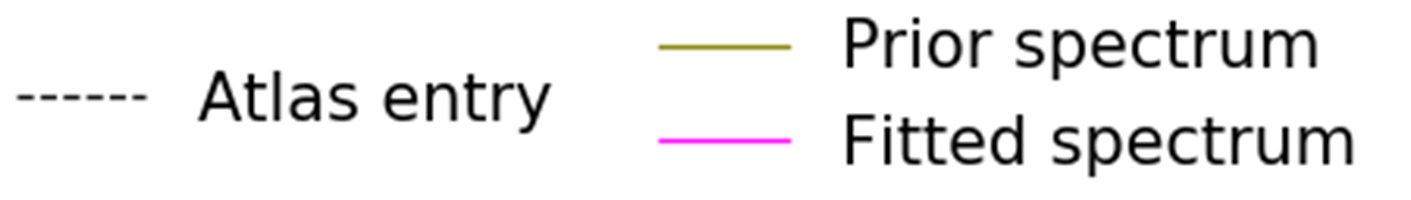
\includegraphics[width=\linewidth]{img/cost_functions_regular_legend.png}
	\end{subfigure} \\
	\begin{subfigure}[t]{0.45\textwidth}
	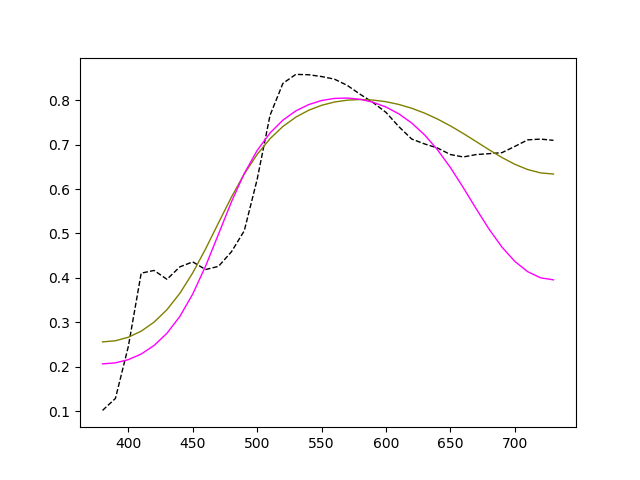
\includegraphics[width=\linewidth]{img/cost_functions_regular_round2.png}
	\caption{Fitting in the second round, i.e. the prior coefficients are the result of ``recomputation'' of the fitted coefficients of an atlas lattice point}
	\label{fig:costFunctionsRegularRound2}
	\end{subfigure} \hspace{0.1em}
	\begin{subfigure}[t]{0.45\textwidth}
		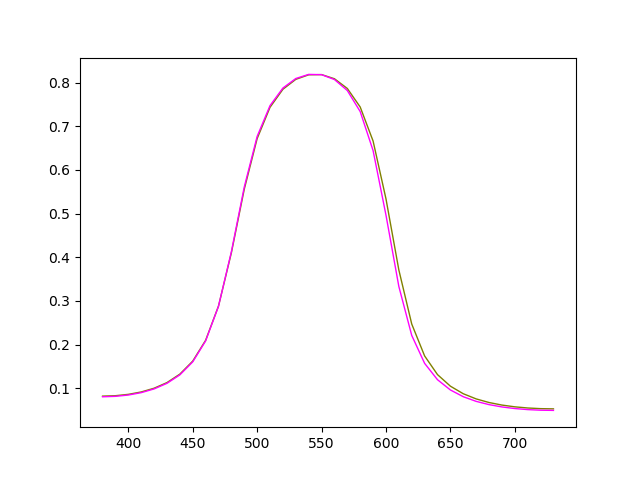
\includegraphics[width=\linewidth,height=0.2\textheight]{img/cost_functions_regular_round8.png}
		\caption{Fitting in round 8/20, where the prior spectrum is that of a regular lattice point}
		\label{fig:costFunctionsRegularRound8}
	\end{subfigure} 
	\caption{Fitting of regular lattice points with 3 cost functions specifying the RGB difference}
	\label{fig:costFunctionsRegularFitting}
\end{figure}

However, when fitting the atlas lattice points (see~\cref{ssec:startingPointsFitting}), the fact that the cost functions do not take the resulting shape of the spectra into account in any way works to our disadvantage. We show an example of this in~\cref{fig:resultsCostFunctions} on the magenta plot, which demonstrates the performance of fitting of atlas lattice points with RGB cost functions only. Although it terminates as successful (as the RGB of the resulting curve is within the fitting threshold of the target RGB), the reflectance curve takes on a sinusoidal shape with a rather high amplitude, therefore losing resemblance to the original curve. This is due to definition of coefficients, which are, in their nature, Fourier coefficients, and are therefore prone to exhibiting this type of behavior. This is mainly perceivable when the color distance $d$ between the atlas entry and atlas lattice point is rather high, as it gives the optimizer enough room to make visible changes in the shape of the reconstructed spectrum before converging below the fitting threshold.
 
Note that we compare the fitted spectra not with the original atlas spectra, but with the spectra that is reconstructed from the original's coefficients to keep track of the optimizer's ability to mimic its input.

\begin{figure}[t]
	\centering
	\captionsetup[subfigure]{font=footnotesize,labelfont=footnotesize}
	\captionsetup[subfigure]{justification=centering}
	\begin{subfigure}[t]{0.70\textwidth}
		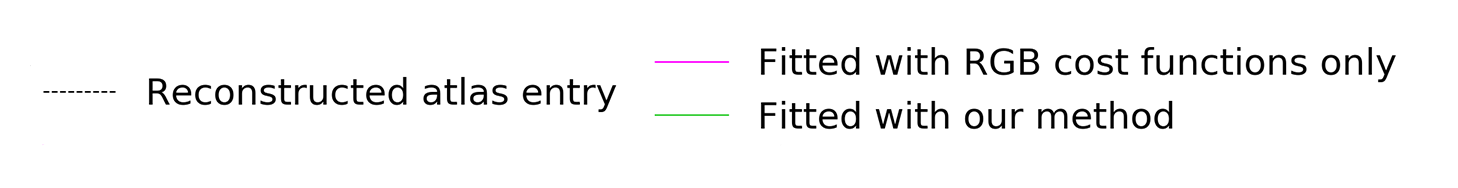
\includegraphics[width=\linewidth]{img/results_costFunctions_legend.png}
	\end{subfigure} \\
	\begin{subfigure}[t]{0.45\textwidth}
		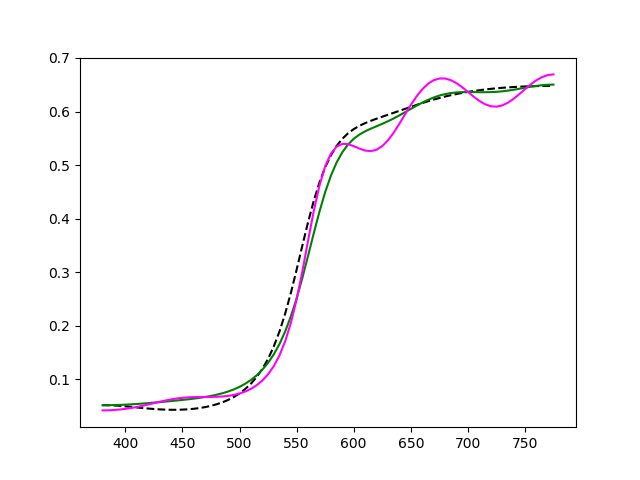
\includegraphics[width=\linewidth]{img/results_costFunctions_orange.png}
		\caption{``orange'' patch of the MCC, $c = 8$, $d = 11.84$}
		\label{fig:resultsCostFunctions_orange}
	\end{subfigure} \hspace{0.1em}
	\begin{subfigure}[t]{0.45\textwidth}
		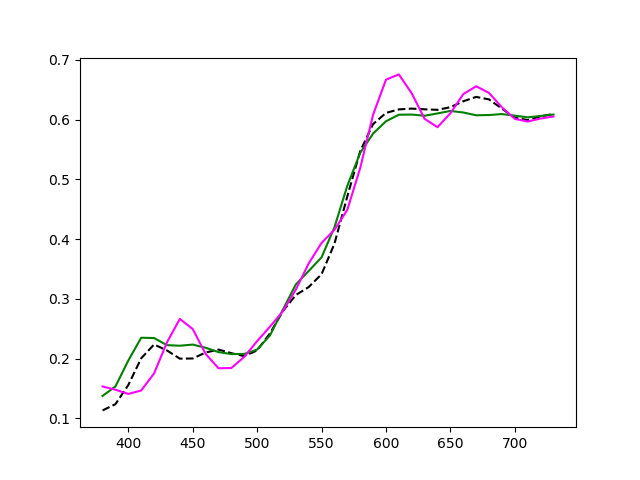
\includegraphics[width=\linewidth]{img/results_costFunctions_mcb0706.png}
		\caption{5YR 7/6 patch of the MBC, $c = 14$, $d = 5.85$}
		\label{fig:resultsCostFunctions_mcb0706}
	\end{subfigure} 
	\vspace{0.5em}\\
	\begin{subfigure}[t]{0.45\textwidth}
		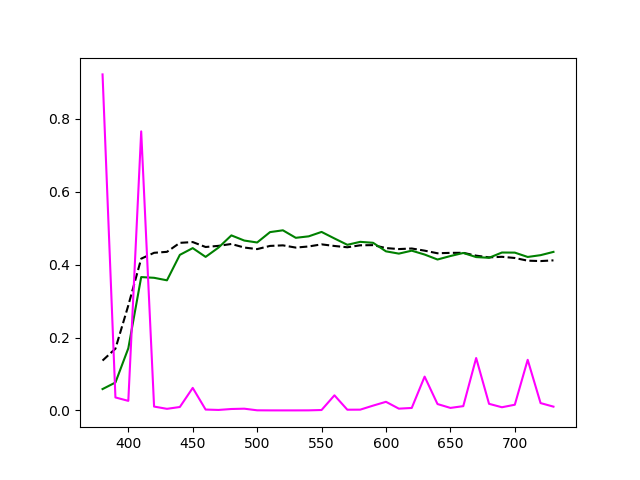
\includegraphics[width=\linewidth]{img/results_costFunctions_mcb0725.png}
		\caption{N 7.25 patch of the MBC, $c = 20$, $d = 12.67$}
		\label{fig:resultsCostFunctions_mcb0725}
	\end{subfigure} \hspace{0.1em}
	\begin{subfigure}[t]{0.45\textwidth}
		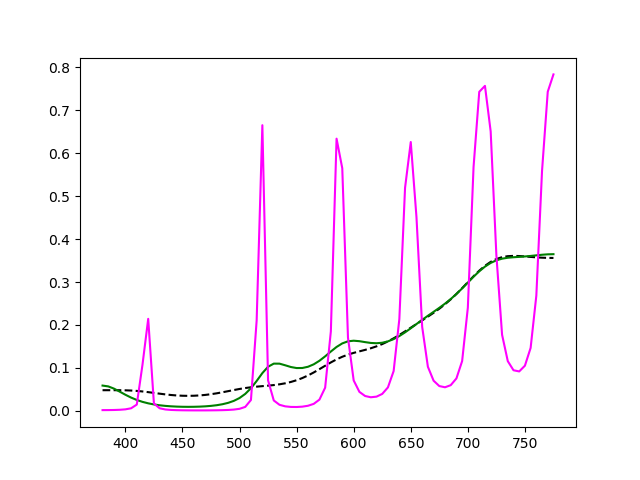
\includegraphics[width=\linewidth]{img/results_costFunctions_darkskin.png}
		\caption{``dark skin'' patch of the MCC, $c = 12$, $d = 11.55$}
		\label{fig:resultsCostFunctions_darkskin}
	\end{subfigure}
	\caption{Comparison between the RGB cost functions and our method for fitting atlas lattice points}
	\label{fig:resultsCostFunctions}
\end{figure}

We therefore conclude that we must incorporate the requirement of curve shape similarity into our cost functions. Following, we review the cost functions that we tried along with their performance.

Firstly, we implemented an approach similar to that for determining the number of coefficients with which to store atlas entries (see ref), i.e. we utilized the color error under a fluorescent illuminant (specifically, FL11). We defined three additional cost functions, each specifying the difference between the original and the reconstructed curve's RGB under the FL11 illuminant in one of the axes. If their values fell below a specific threshold, we terminated the fitting process as successful, if not, we increased the threshold and tried again.

Although this approach was successful on average (the average threshold was around $t = 0.025$), on occasion, the threshold often needed to be increased to values so high that it became obsolete. Using only one error, either the Euclidean distance or the Delta E error, caused similar issues.

Therefore, we decided to focus on the actual distance between the two curves. Our first attempt consisted of defining one residual per wavelength sample specifying the absolute distance between the two spectra at said wavelength (as the least square error proved to perform worse). We examined the performance of both around 360 residuals (i.e. 1nm increment between samples) and 36 residuals (10nm increment, as defined in most color atlases) when used alongside the 3 already defined RGB residuals. For $c \le 9$, both of these options performed reasonably well. When fitting more coefficients, the sufficient threshold was, on average, around $t = 0.0096$, both before and after the introduction of our improvement of optimizing only first 4 coefficients, and although its maximum ended up being $t = 0.23$, overall, this method outperformed the previous one.

As we suspected that the failures were caused by the abundance of cost functions, we summed up their values and saved them into a single residual, which, when divided by the number of spectral samples, represented the average error per sample.

As the importance of curve samples in terms of proper color reconstruction is mainly placed on their middle (at around 550nm), we attempted to add a heuristic-based weighting factor in an effort to focus on minimizing the distance between the two curve there. However, we did not succeed in improving our results, and we therefore dropped the experiment and examined the performance without weighting the values.

Such an approach substantially outperformed the previous ones, and even more after we decided to specify the absolute error rather than the least square error. The average error ended up being only about $d = $, and, of yet, no entry requiring $d > $ has been encountered. Therefore, we concluded that the optimal solution to our problem is to set 4 residuals, 3 specifying the RGB difference, and 1 specifying the average distance per sample.

We present some of the results achieved with our cost functions on the green plot in~\cref{fig:resultsCostFunctions}, where we compare them to fitting with RGB cost functions only. In~\cref{fig:resultsCostFunctions_mcb0725} and~\cref{fig:resultsCostFunctions_darkskin}, we specifically focus on the most problematic spectra with the highest distance $d$ between the atlas lattice point and the atlas entry.

Although our approach substantially reduces the appearance of sinosidual-like behavior, it does not diminish it completely. It can be observed especially for atlas lattice points with $c > 14$ (see~\cref{fig:resultsCostFunctions_mcb0725}). This is due to the fact that we optimize only the first 4 coefficients, which, in their nature, are prone to creating such patterns.

Another drawback of our approach is the substantially larger time complexity, especially if improvement heuristics need to be applied. By examining the scope of the optimizer and utilizing its options further, or maybe even resorting to a different optimizer, we might be able to improve upon both the time complexity, and the resulting spectral shape.

However, as the runtime is not the focus of this thesis and as the resulting shapes are satisfactory for the purposes of this these, we focused our efforts elsewhere and leave these improvements for future work.

 However, as that is not the focus of this thesis, we leave the improvements in time complexity for further work.


\subsection{Number of moments}
 
Maybe add a section about unfittable cubes?

However, correct round-trips are not the only factor we need to take into consideration when fitting the cube. We also need to focus on both the \emph{smoothness of the resulting spectra} and the \emph{behavior of the optimizer} under the current technique.

The smoothness of the spectra is especially important for the interpolation process that takes place during the rendering. Interpolating multiple spiky, non-similar spectra would result in similarly uneven spectra, which, in addition to incorrect color, may be susceptible to extreme metameric artifacts.  

The behavior of the optimizer also plays a big role. During the optimization, it takes into account only the resulting RGB of the curve rather than the shape of the curve itself. Therefore, it does not aim for a curve with a similar shape than its neighbor, which may likewise cause issues during the interpolation.

When we fit from the middle, we only aim for the smoothness of the resulting spectra and for the behavior of the optimizer. We therefore want as less coefficients as possible and, as we do not care about round trips, we can use any of the techniques available.

We already said that using 9 coefficients is unecessary, as 3 already create rather smooth spectra that is way better for interpolation. However, we here find out that it is not only unnecessary but extremely discouraged. We can see in the image how the fitting proceeds. It amplifies the already existing wave-like patterns, exhibiting the same behavior as it did during atlas fitting, which is caused by the cost functions not considering the shape of the resulting spectra. By allowing only three coefficients, we limit the optimizer so it must create smooth spectra and it cannot create crazy shapes. Additionaly, it is better for performance - fiting of a 9-coefficients takes around blabla, while fitting 3 takes blabla. We provide measurements here? of performance

Although we cannot control shape, we can control smoothness. We want smooth spectra both for interpolation purposes and because smooth spectra is less prone to metameric artifacts, see chapter 1.

The behavior we talked about before of the optimizer is a problem 
It would be extremely beneficial for the

For middle fitting, we always recommend 2 moments, 3 coeffs due to the runtime. Moreover, they are very smooth but not straight which is ideal for our purposes. Obviously, we can fit with higher but that takes a lot of time and does not provide any advantage. The default setting is therefore 3 coefs, 2 moments.

Obviously, fitting with these causes metameric artifacts, similar to the ones created by sigmoid, we show these in PICTURE. We can also show metameric artifacts when fitting with more? (try this maybe)

Another slight trick is to use a lower number of coefficients - we therefore do not get as big artifacts because we cannot possibly reconstruct such crazy spectra with low number of coefficients. 

The optimizer is always faster for lower number of coefficients as it does not need to change them up as much. Also faster but does not change them so much SO it results in spectrum that is similar to the first one. However, we cannot possibly simulate the curve with only the limited number of coefficients, the table says so. Therefore we must find something in the middle. We try not to focus on performance here because obviously, fitting anything that is higher than 32 takes hours and we want to have it look the best way we can.

\section{Performace}

heuristics performance, overall runtime of the cube

\section{Rendering}

- which technique gives the best results (metamerism results)


Also mention that it is multi-threaded and performance is not really a priority - the cube has to be created only once and then can be reused as much as the artists need.
